%!TEX root = ../proteoform_suite_manual.tex
%---------------------------------------------------------------------
%	PROTEOFORM FAMILIES
%---------------------------------------------------------------------

\section{Proteoform Families}

\subsection{Overview}

On this page, accepted experiment-theoretical and experiment-experiment pairs are joined to construct proteoform families. Experimental proteoforms are identified by intact-mass analysis; beginning with each theoretical proteoform in each family, connections between proteoforms are traced to identify proteoforms first from experiment-theoretical pairs and then from subsequent experiment-experiment pairs. Decoy proteoform families are constructed from experiment-decoy and experiment-false pairs and are used to calculate a global false discovery rate for intact-mass proteoform identifications. A script for Cytoscape\supercite{Shannon2003,Smoot2011} can be exported to visualize proteoform families as a network of nodes (proteoforms masses) and edges (mass differences between proteoforms). 

\subsection{Run Page}
\begin{itemize}
\item The Experiment-Theoretical Comparison and Experiment-Experiment Comparison pages must be run before running this page.
\item Set all parameters as desired for current analysis (see below)
\item Click Run Page button (top right)
\end{itemize}

\subsection{Set Parameters}
\begin{figure}[h]
\centering
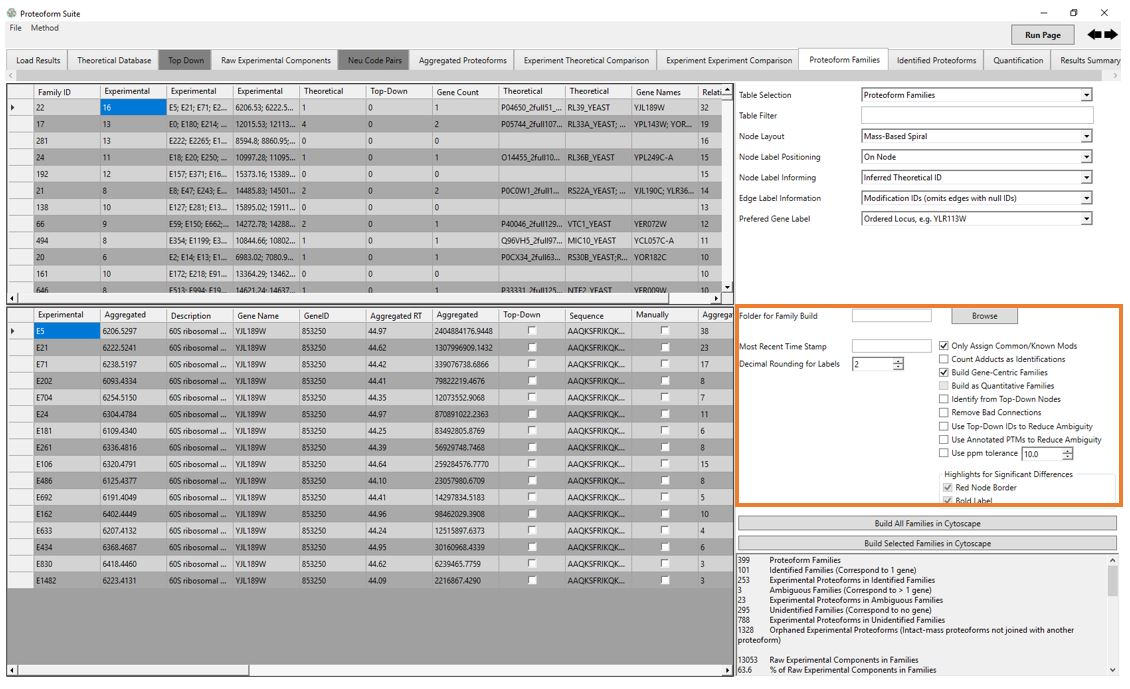
\includegraphics[scale=0.5]{figures/families1.jpg}
\end{figure}
\begin{itemize}
\item Folder for Family Build: folder to build scripts to visualize proteoform families in Cytoscape
\item Most Recent Time Stamp: time stamp that will be in the filename of scripts to visualize proteoform families in Cytoscape
\item Decimal Rounding for Labels: number of decimal places to round labels in visualized proteoform families in Cytoscape
\item Only Assign Common/Known Mods: if checked, intact-mass identifications will only be made for common modifications or for modifications annotated for that theoretical protein in UniProt
\item Count Adducts as Identifications: if checked, adducts (oxidation, sulfate adducts, SDS adducts) will be counted as unique identifications
\item Build Gene-Centric Families: if checked, all proteoforms connected to theoretical proteoforms from the same gene will be grouped into the same proteoform family
\item Build as Quantitative Families: if checked and if quantification was performed, quantitative proteoform families will be built (with pie charts for each experimental proteoform showing abundance ratios)
\item Identify from Top-Down Nodes: if checked, top-down proteoforms in additional to theoretical proteoforms will be used as starting points for identification in proteoform families. This requires high-quality top-down identifications to prevent high false discovery rate
\item Remove Bad Connections: if checked, connections between proteoforms in identified families that do not lead to identification will be removed, unaccepting the experiment-theoretical or experiment-experiment pairs
\item Use Top-Down IDs to Reduce Ambiguity: if checked, top-down IDs will be used to reduce ambiguity in intact-mass identifications; identifications from theoretical proteoforms confirmed by top-down will be prioritized
\item Use Annotated PTMs to Reduce Ambiguity: if checked, annotated PTMs in UniProt will be used to reduce ambiguity in intact-mass identifications; identifications with an annotated PTM will be prioritized
\item Use ppm tolerance: if checked, this ppm tolerance will be used when making intact-mass identifications in proteoform families
\item Highlights for Significant Differences: if checked, a red node border and bold label will be used in quantitative proteoform families to highlight experimental proteoforms with statistically significant quantitative differences
\end{itemize}
\pagebreak
\subsection{Results}
\begin{itemize}
	\item Proteoform Families table: the top table displays all constructed proteoform families
	\begin{figure}[h]
\centering
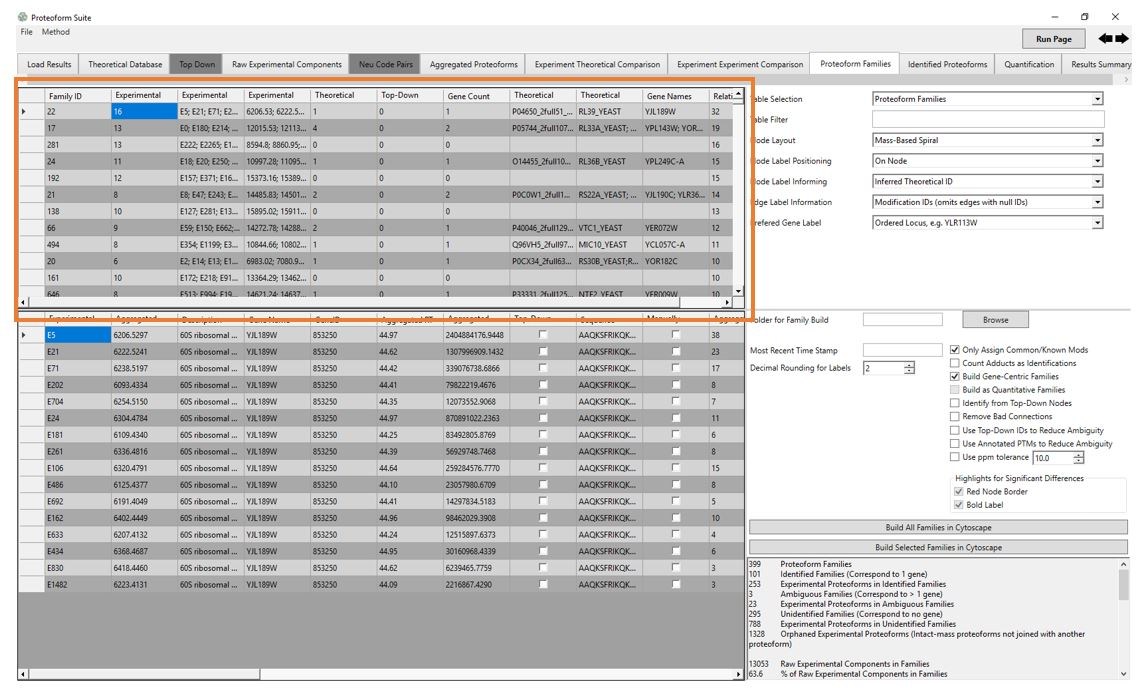
\includegraphics[scale=0.5]{figures/families2.jpg}
\end{figure}
\begin{itemize}
	\item Family ID: unique ID assigned by Proteoform Suite for this proteoform family
	\item Experimental Proteoforms: number of experimental proteoforms in this proteoform family
	\item Experimental Accessions: semi-colon separated list of accessions for experimental proteoforms in this proteoform family
	\item Experimental Aggregated Masses: semi-colon separated list of masses for experimental proteoforms in this proteoform family
	\item Theoretical Proteoforms: number of theoretical proteoforms in this proteoform family
	\item Top-Down Proteoforms: number of top-down proteoforms in this proteoform family
	\item Gene Count: number of genes in this proteoform family. Families with more than 1 gene are ambiguous and families with no genes are unidentified
	\item Theoretical Accessions: semi-colon separated list of accessions for theoretical proteoforms in this proteoform family
	\item Theoretical Names: semi-colon separated list of protein names for this proteoform family
	\item Gene Names: semi-colon separated list of gene names in this proteoform family
	\item Relation Count: number of proteoform relations in this family (experiment-theoretical pairs and experiment-experiment pairs)
\end{itemize}
\item Proteoforms table: the bottom table displays proteoforms for the proteoform family selected in the Proteoform Families table. 
	\begin{figure}[h]
\centering
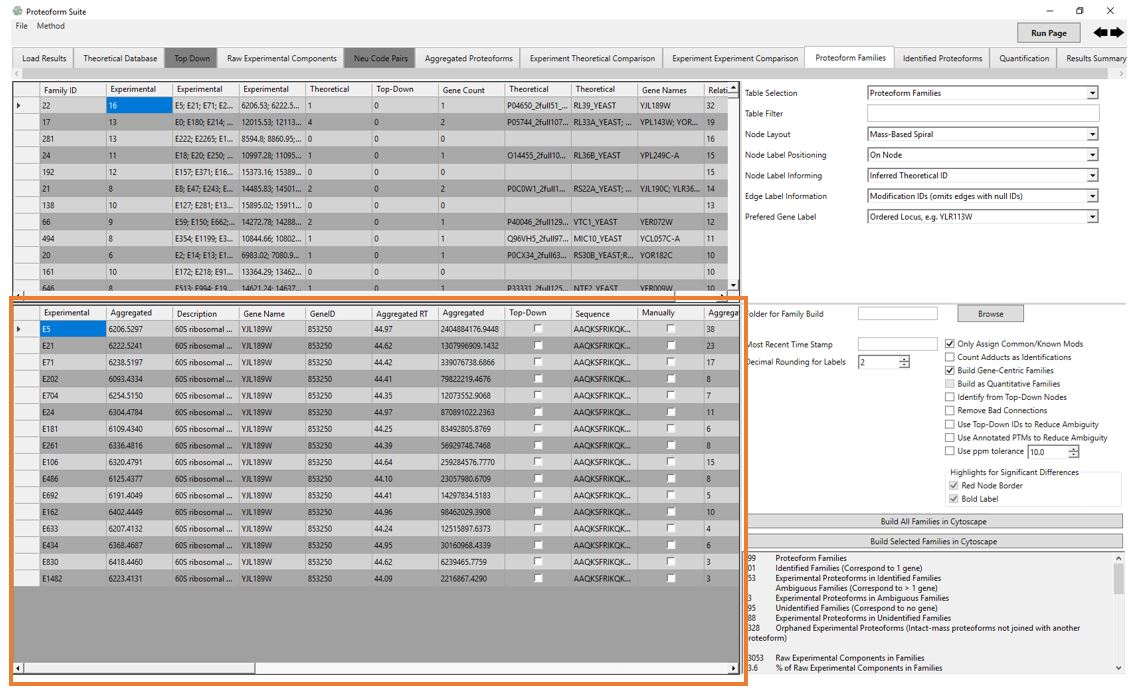
\includegraphics[scale=0.5]{figures/families3.jpg}
\end{figure}
\begin{itemize}
\item If the Experimental Proteoforms, Experimental Accessions, or Experimental Aggregated Masses columns are selected, the experimental proteoforms for the selected family will be displayed. See the Aggregated Proteoforms table in the \textbf{Aggregated Proteoforms} section for column descriptions. 
\item If the Theoretical Proteoforms, Theoretical Accessions, or Theoretical Names Columns are selected, the theoretical proteoforms for the selected family will be displayed. See the Theoretical Proteoforms table in the \textbf{Theoretical Proteoforms} section for column descriptions.
\item If the Top-Down Proteoforms column is selected, the top-down proteoforms for the selected family will be displayed. See the Top-Down Proteoforms table in the \textbf{Top-Down Proteoforms} section for column descriptions.
\item If the Relation Count column is selected, the proteoform relations in the selected family will be displayed. See the Experiment-Theoretical Pairs table in the \textbf{Experiment-Theoretical Comparison} section and the Experiment-Experiment Pairs table in the \textbf{Experiment-Experiment Comparison} section for column descriptions.
\end{itemize}
\item Table Selection: this drop-down box changes which proteoform families are displayed (target or decoy communities). Can also observe theoretical proteoforms and GO Terms
\item Table Filter: filter the Proteoform Families table (top left) by any entered text
\item Node Layout: this drop-down box changes the node layout in visualized proteoform families in Cytoscape
\item Node Label Positioning: this drop-down box changes the position of node labels in visualized proteoform families in Cytoscape
\item Node Label Informing: this drop-down box changes the node label information in visualized proteoform families in Cytoscape
\item Edge Label Information: this drop-down box changes the edge label information in visualized proteoform families in Cytoscape
\item Preferred Gene Label: this drop-down box changes the gene label information in visualized proteoform families in Cytoscape
\item Build All Families in Cytoscape: exports scripts for Cytoscape to visualize all proteoform families
\item Build Selected Families in Cytoscape: exports scripts for Cytsocape to visualize proteoform families selected in the Proteoform Families table
\item The text box at the bottom right of the page displays information about the results. See the \textbf{Results Summary} section for a description of each result
\end{itemize}